\documentclass[12pt]{article}
\usepackage{graphicx}
\usepackage{amssymb}
\usepackage{epstopdf}
\usepackage{amsmath}
\usepackage{multicol}
\usepackage{tcolorbox}
\usepackage{geometry}
\usepackage{enumitem}
\usepackage{fancyhdr}
\usepackage{tabu}

\DeclareGraphicsRule{.tif}{png}{.png}{`convert #1 `dirname #1`/`basename #1 .tif`.png}

\textwidth = 6.5 in
\textheight = 9 in
\oddsidemargin = 0.0 in
\evensidemargin = 0.0 in
\topmargin = -23pt
\headheight = 0.0 in
\headsep = 0.0 in
\parskip = 0.2in
\parindent = 0.0in
\pagestyle{fancy}
\pagenumbering{gobble}

\newtheorem{theorem}{Theorem}
\newtheorem{corollary}[theorem]{Corollary}
\newtheorem{definition}{Definition}
%\includegraphics [height=50mm, width=50mm]{PathInt.jpg}
\title{Title} 

\begin{document}
%INSTRUCTOR NOTES
%Question 2(c) and (g) are very similar. (f) is a hard one.
%There might not be time for #3

Name:
 \begin{center}\large{Trigonometry Review}\end{center}
\begin{enumerate}
\item Sketch each angle listed below in standard position on the unit circle. Then give the exact coordinates of each of the angle.\\
\noindent\begin{minipage}{0.3\textwidth}% adapt widths of minipages to your needs
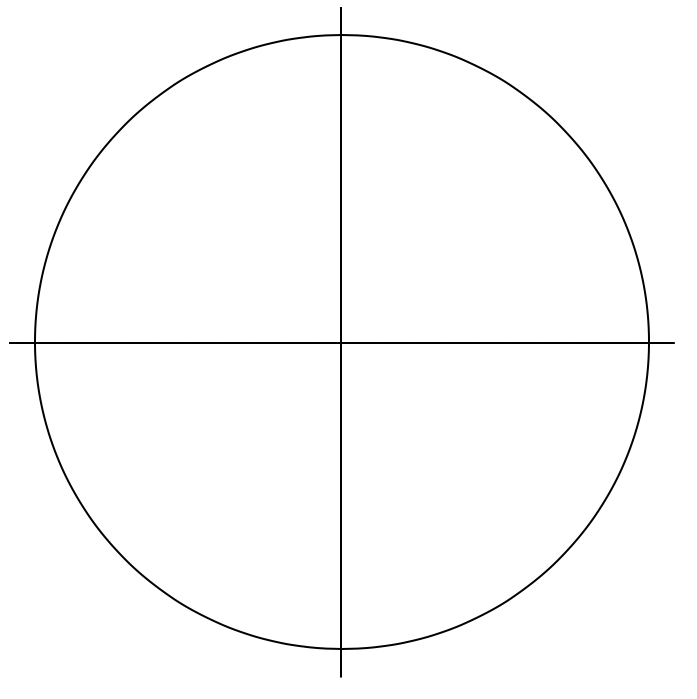
\includegraphics [height=50mm, width=50mm]{Trig_Blank_Unit}
\end{minipage}%
\hspace{40mm}
\begin{minipage}{0.6\textwidth}
(a) $\theta = \pi$; $\big(~~~,~~~\big)$\\

\vspace{5mm}

(b) $\theta = \frac{2\pi}{3}$; $\big(~~~,~~~\big)$\\

\vspace{5mm}

(c) $\theta =- \frac{\pi}{4}$; $\big(~~~,~~~\big)$\\


\end{minipage}

\item Suppose $\theta$ is an angle whose terminal edge intersections the unit circle at the point $(x,y)$. If $x=-\frac{1}{5}$ and $(x,y)$ is in the third quadrant, find each of the following:\\
\begin{multicols}{3}
\begin{enumerate}[itemsep=2cm]
\item $\cos \theta = $
\item $\sin \theta = $
\item $\tan \theta = $
\item $\sec \theta = $
\item $\csc \theta = $
\item $\cot \theta = $
\end{enumerate}
\end{multicols}
\vspace{20mm}
\item What is the difference between $\sin^2 x$, $\sin x^2$, $(\sin x)^2$, and $\sin(\sin(x))$? Consider using a graphing utility to check your reasoning.

\vfill
\newpage 
\rhead{Trigonometry Review}

\item Consider the sinusoidal graph below. \\
\noindent\begin{minipage}{0.3\textwidth}% adapt widths of minipages to your needs
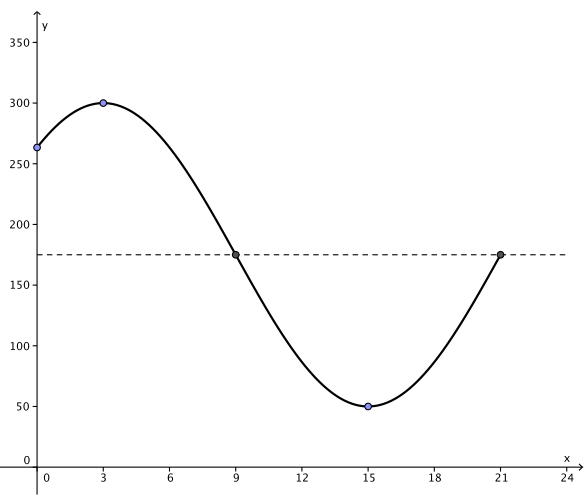
\includegraphics [height=70mm, width=80mm]{Trig_Sinusoidal}
\end{minipage}%
\hspace{40mm}
\begin{minipage}{0.4\textwidth}
(a) Determine an equation of a cosine function that produces the graph below. You mind find it helpful to determine things like the amplitude, period, and midline of the function. Double-check your answer by graphing it or testing a few points.
\vspace{5mm}

(b) Now find a sine function that produces the same graph.
\end{minipage}
\vfill

\item Find all values of $x$ in the interval $[0, 2\pi]$ that satisfy the following equations. If you deleted the condition that your answer must lie in the interval $[0, 2\pi]$, would your answer change? If yes, how?
	\begin{enumerate}
	\item  $\sin(x)=\frac{\sqrt{3}}{2}$
	\vfill
	\item $5\tan(x)+3=-2$
	\vfill
	\item $\sin(2x) = \cos x$
	\vfill
	\end{enumerate}







\end{enumerate}
\end{document} 

%%%%%%%%%

\underline{\hspace{3cm}}
%Warm-up
\begin{tcolorbox}
\textbf{Warm-up: } Solve the following equations for $t$.
\begin{multicols}{2}
\begin{enumerate}[itemsep=1cm]
\item $(t+1)^2=9$
\item $tx+x^2=5$
\end{enumerate}
\end{multicols}
\end{tcolorbox}

%MINIPAGE
\noindent\begin{minipage}{0.3\textwidth}% adapt widths of minipages to your needs
try 1
\end{minipage}%
\hspace{40mm}
\begin{minipage}{0.6\textwidth}
a) $f'(2)=$\\\

b) $f'(4)=$\\

c) $f'(6)=$\\

d) $f'(7)=$\\

e) $f'(8)=$
\end{minipage}


%table
\begin{tabu} to 0.8\textwidth { X[c] | X[c]  X[c] X[c]  X[c] }
 
 $t$ & 0 & 1 & 2 & 3 \\
 \hline
 $f(t)$ & 2 & 3 & 1 & 1 \\
  $g(t)$ & 3 & 1 & 2 &  \\
   $f(g(t))$ &  &  & & 2 \\
 $g(f(t))$ &  &  &  &  \\
\end{tabu}